The main result of this paper is that we can approximate $\bn^{MAP}$ in \emph{linear} time, whereas an exact solution would require exponential time. Fig. \ref{fig:wiener} shows two examples of running the FAND filter on simulated data.  On the left, the data is simulated according to Eqs. \eqref{eq:F} and \eqref{eq:C}, with a low expected firing rate (5 Hz).  The FAND filter performs very well (middle left panel): when spikes occured (gray downward facing triangles), the FAND filter's output is relatively high, and in the absence of a spike, the FAND filter's output is relatively low. The height of the ``spikes'' in $\bn^{FAND}$ can be thought of as the probability of a spike having occurred.  The Wiener filter does not perform as well on this data.  Specifically, $\bn^{Wiener}$ exhibits a ``ringing'' effect, in which the inference oscillates around zero in the absence of true spikes.  This occurs because negative spikes improve the inference, if negative spikes are allowed.  By constraining our inference to be non-negative (for the FAND filter), we completely circumvent this problem.  

It is unsurprising that the FAND filter significantly outperforms the Wiener filter when spiking is sparse, given that the exponential is a much better approximation to the Poisson in this regime (c.f. Figure \ref{fig:dist_comp}).  However, even in the fast firing rate scenario, where the Gaussian approximation is far more accurate, the FAND filter performs relatively well, as depicted in the right panels of Figure \ref{fig:wiener}.  Note however that the computational time for computing the FAND filter scales linearly with $T$, i.e. is $O(T)$, whereas the \nai ve implementation of the Wiener filter requires $O(T \log T)$ (but see Appendix \ref{sec:app} for an implementation of the Wiener for that only requires $O(T)$).  

\begin{figure}[H]
\centering 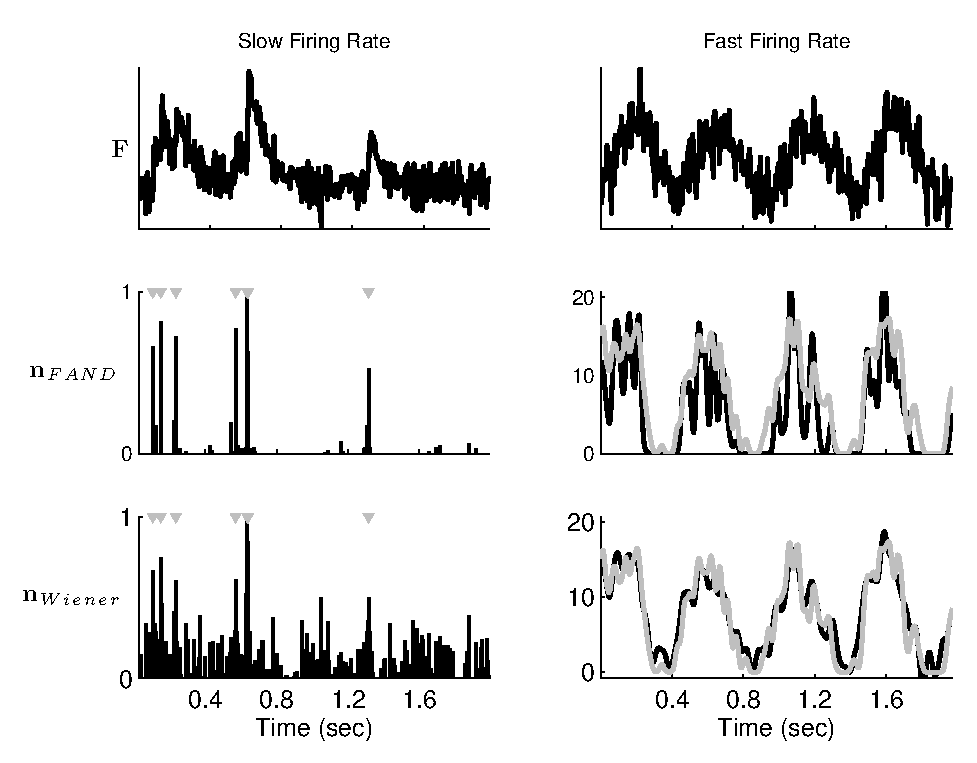
\includegraphics[width=.9\linewidth]{../figs/example_sim}
\caption{A simulation demonstrating the performance of the FAND filter in different firing regimes. The left panels show that in the sparse firing regime, the FAND filter outperforms the Wiener filter in terms of SNR.  This follows because an exponential is a closer approximation to a Poisson than a Gaussian, when spiking is sparse. The right panels show that both approximations are good in the fast firing regime. Top left panel: fluorescence time series for a neuron with a slow firing rate.  Middle left panel: the FAND filter's inferred spike train.  Bottom left panel: Wiener filter's inferred spike train.  Note that (i) the Wiener filter does not impose a non-negativity constraint, and (ii) the effective SNR of the Wiener filter in this example is worse than the FAND filter's.  Top right panel: same as top left panel, for a neuron with a high firing rate.  Middle right panel: the FAND filter's inferred spike train smoothed with a Gaussian kernel for visualization purposes (black line), and the true spike train smoothed with the same Gaussian kernel (gray line).  Bottom right panel: same as middle right panel, but with the Wiener filter. Parameters for left panels: same as in Figure \ref{fig:schem}.  Parameters for right panels: same as Figure \ref{fig:schem}, except: $\sig=8$ photons, $\lam=500$ Hz.} \label{fig:wiener}
\end{figure}

To quantify the relative quality of these inference algorithms in the sparsely spiking regime, we compute the effective signal-to-noise ratio (eSNR), defined as the average squared magnitude of the inferred spiked during frames in which there was a spike, divided by the same quantity computed in frames lacking a spike.  The left panels of Figure \ref{fig:stats} show how the eSNR varies as a function of the magnitude of the noise on observations (top left panel), and the expected firing rate (bottom left panel).  The FAND filter's inference (blue line) dominates the Wiener filter (red line), as well as the post-hoc half wave rectifier Wiener filter, $[$Wiener$]_+$ (green line), and a simple dF/F (turquoise line).  

When the neuron is exhibiting a high firing rate, we compute the mean-squared error (MSE) between the inferred number of spikes, and the true number of spikes.  The top right panel of Figure \ref{fig:stats} shows that when noise is relatively low, the FAND filter performs about as well as the Wiener filter.  However, in the high noise regime, the Wiener filter clearly outperforms the FAND filter.  

To verify that both our implementations of the FAND filter and the Wiener filter scale linear with respect to the number of image frames, the bottom right panel of Figure \ref{fig:stats} shows a such a linear relationship (on a log-log scale).  

The take home message from Figure \ref{fig:stats} is that when we expect $<1$ spike per frame, the FAND filter significantly outperforms the Wiener filter, regardless of variance of the observation noise.  Furthermore, because of our linear time algorithm, filtering around 50,000 image frames requires only about 1 second on a standard Apple laptop.  Below, we improve on our inference quality by generalizing our model in a number of ways.

%This suggests that when data is very noisy, and firing rate is expected to be relatively high (e.g., $>10$ spikes per frame), the Wiener filter should be the filter of choice.  

%a number of distance measures between $\bn$ and our inferred $\hbn$: (a) cross correlation, (b) mean square error, and (c) signal-to-noise ratio (see Section \ref{sec:ass} for details). Figure \ref{fig:stats} (top panels) shows how the various algorithms (FAND in blue, Wiener in red, half-wave-rectified Wiener in green, dF/F in turquise) perform according to each of these measures, as a function of the noisiness of the data. Clearly, regardless of the variance of the noise, the FAND filter outperforms all other approaches considered here.   On the contrary, in the high firing rate regime, the Wiener filter is optimal, as expected (lower left panels).  Note that SNR is only an appropriate measure when there is at most one spike per image frame.  Finally, do demonstrate that our algorithms are indeed linear in the number of time steps, we show how computational time scales with $T$ (lower right panel) for each algorithm.


\begin{figure}[H]
\centering 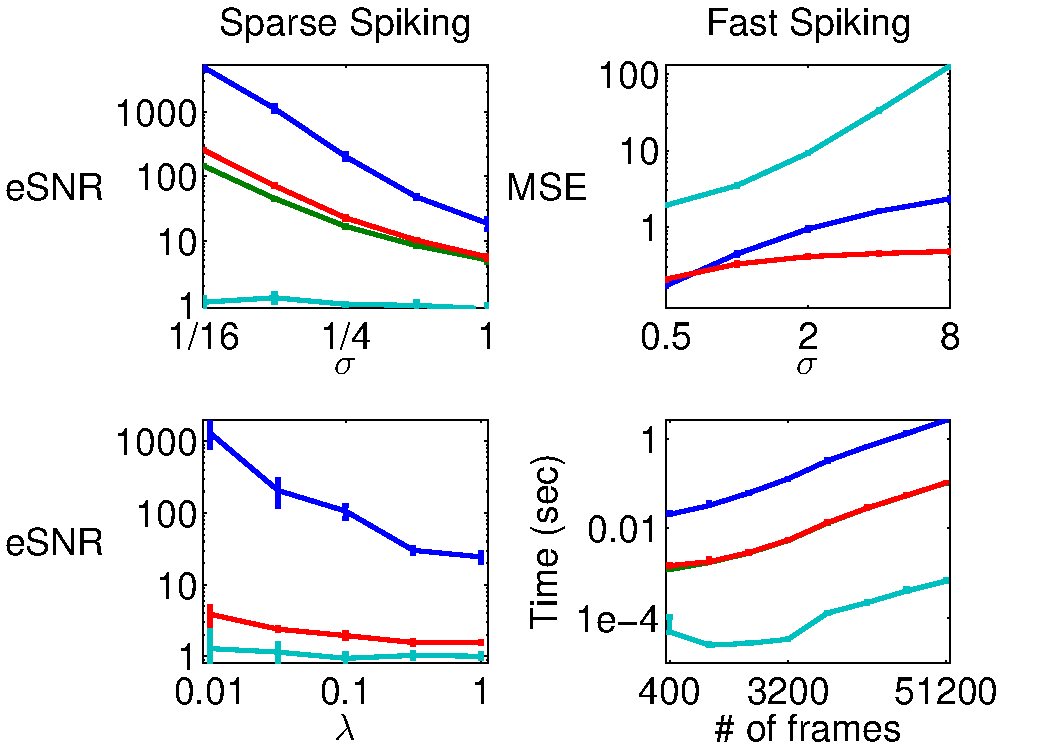
\includegraphics[width=.9\linewidth]{../figs/stats}
\caption{Quantitative assessment of the FAND filter's inference quality and speed.  The left columns show that the FAND filter outperforms the Wiener filter in terms of eSNR --- Eq. \eqref{eq:SNR} --- regardless of variance of observation noise (top) and expected firing rate (bottom).  The top right panel show that when noise is low, even when firing rates are relatively (e.g. $\lam \Del=20$ Hz), the FAND filter and Wiener filter both perform well.  Both algorithms scale linearly with the number of image frames, meaning that it takes about 1 second of computational time per 50,000 image frames, using either algorithm.  %The FAND filter outperforms other approaches when neurons are spiking sparsely, and the Wiener filter is best when neurons have firing rates.  Both our algorithms perform in linear time.  Specifically, a movie of 50,000 frames can be filtered in about 1 second, using either our implementation of the FAND or Wiener filter.  To ascertain inference quality, we use (a) correlation coefficient (left panels), (b) mean square error (middle panels), and (c) effective signal-to-noise ratio (top right panel),see Section \ref{sec:ass} for definitions.  The top panels show that, using all three measures, when spikes are sparse, the FAND filter (blue line) outperforms the Wiener filter (red line), $[$Wiener$]_+$ (green line), and dF/F (turquoise line).  The bottom left panels show that the Wiener filter outperforms the FAND filter for fast spiking neurons.  Note that $[$Wiener$]_+$ is not visible in the bottom panels, as it is completely under the Wiener filter.  Further, SNR is not an appropriate measure in this regime.  The bottom right panel shows that all algorithms are require $O(T)$ time, whereas a \nai ve implementation of non-negative deconovlution would require $O(T^3)$ time, and a \nai ve implementation of the Wiener filter would require $O(T \log T)$ time. Note that both axes in this plot are on a log scale.  
Simulation details: 5 simulations for each point on all the plots, mean (solid line) and standard deviation (bars) are shown for each.  Parameters: $\Del = 0.005$ sec, $\alpha=1$, $\beta=0$.  Top left: $\lam=1$ Hz, $\tau=1$ sec.  Top right: $\lam=10$ Hz, $\tau=1$ sec.  Bottom left: $\sig=0.25$, $\tau=0.5$ sec.  Bottom right: $\sig=0.25$, $\tau=0.1$ sec, $\lam=1$ Hz.} \label{fig:stats}
\end{figure}


% To quantify the relative quality of these inference algorithms, Table \ref{tab:1} shows $R_{\hbn}$ and AUC for simulations like these, as well as computational time.  Clearly, the FAND filter is preferable to the Wiener filter, in that the FAND filter's performance is at least as good as the Wiener filter's, and requires less time.  
% 
% \begin{table}
% \caption{Simulated performance} \label{tab:slow}
% \centering
% \begin{tabular}{c|c|c|c|c|c}
% \multicolumn{6}{c}{Slow Firing Rate} \\ %\hline
% %Filter 			& $R_{\hbn}$ 	& $MSE$ 		& $SNR$ 		& $AUC$ & Time \\ \hline
% Filter & $R_{\hbn}$ & $MSE$ & $SNR$ & $AUC$ & Time \\ \hline 
FAND& 0.920 (0.009) & 0.006 (0.001) & 396.256 (91.462) & 6.315 (0.289) & 0.495 (0.020) \\ 
Wiener& 0.552 (0.012) & 0.024 (0.002) & 19.337 (1.508) & 6.485 (0.462) & 0.022 (0.001) \\ 
$[$Wiener$]_+$& 0.670 (0.010) & 0.017 (0.001) & 29.801 (2.436) & 6.485 (0.462) & 0.022 (0.001) \\ 
dF/F& -0.029 (0.009) & 0.067 (0.006) & 1.109 (0.222) & 0.853 (0.089) & 0.000 (0.000)
% %\end{tabular}
% %\end{table}
% \\ \hline \\
% %\begin{table}
% %\caption{Fast Firing Rate} \label{tab:fast}
% %\centering
% %\begin{tabular}{c|c|c|c|c|c}
% \multicolumn{6}{c}{Fast Firing Rate} \\ %\hline
% %Filter 			& $R_{\hbn}$ 	& $MSE$ 		& $SNR$ 		& $AUC$ & Time \\ \hline
% Filter & $R_{\hbn}$ & $MSE$ & $SNR$ & $AUC$ & Time \\ \hline 
FAND& 0.752 (0.005) & 67.689 (1.703) & NaN (NaN) & NaN (NaN) & 0.765 (0.016) \\ 
Wiener& 0.916 (0.001) & 15.323 (0.141) & NaN (NaN) & NaN (NaN) & 0.243 (0.005) \\ 
$[$Wiener$]_+$& 0.916 (0.001) & 15.323 (0.141) & NaN (NaN) & NaN (NaN) & 0.243 (0.005) \\ 
dF/F& 0.006 (0.005) & 385.433 (2.399) & NaN (NaN) & NaN (NaN) & 0.000 (0.000)
% \end{tabular}
% % }
% % \end{multicols}
% \end{table}

Finally, often one is interested in understanding the relationship between spike trains and the environment.  Therefore, we simulated a neuron whose spiking activity was a function of a 5-dimensional external stimulus.  More specifically, we let $\lam_t = \bk\T \bx_t$, where $\bk$ is a 5-dimensional linear kernel, $\bx_t$ is the stimulus at time $t$, and $P(n_t)=$Poisson($\lam_t \Del$).  We then computed the maximum likelihood estimate of the linear kernel, $\hbk=\hbn \bx\T (\bx \bx\T)^{-1}$.  Importantly, the simulation was constructed to incorporate both sparse spiking and fast spiking periods, much like sensory neurons have periods of quiescence, followed by stimulus driven bursts.  Thus, neither the FAND filter nor the Wiener filter's assumptions are entirely appropriate. Figure \ref{fig:kernel} shows the results of this simulation.  The true kernel, kernel estimated using the true spike times, and kernel estimated using the FAND filter, are nearly overlapping (black, gray, and blue lines, respectively).  The kernel estimated using the Wiener filter output, however, is effectively flat (red line). Post-hoc half-wave rectification of the Wiener filter output does not improve its ability to estimate this kernel (green line --- completely obscured by the unrectified Wiener filter output).  Finally, dF/F does not yield anything useful at all (turquoise line).  This simulation provides further evidence of the quantitative advantage of utilizing the FAND filter before performing an analysis on calcium fluorescence data.

\begin{figure}[H]
\centering 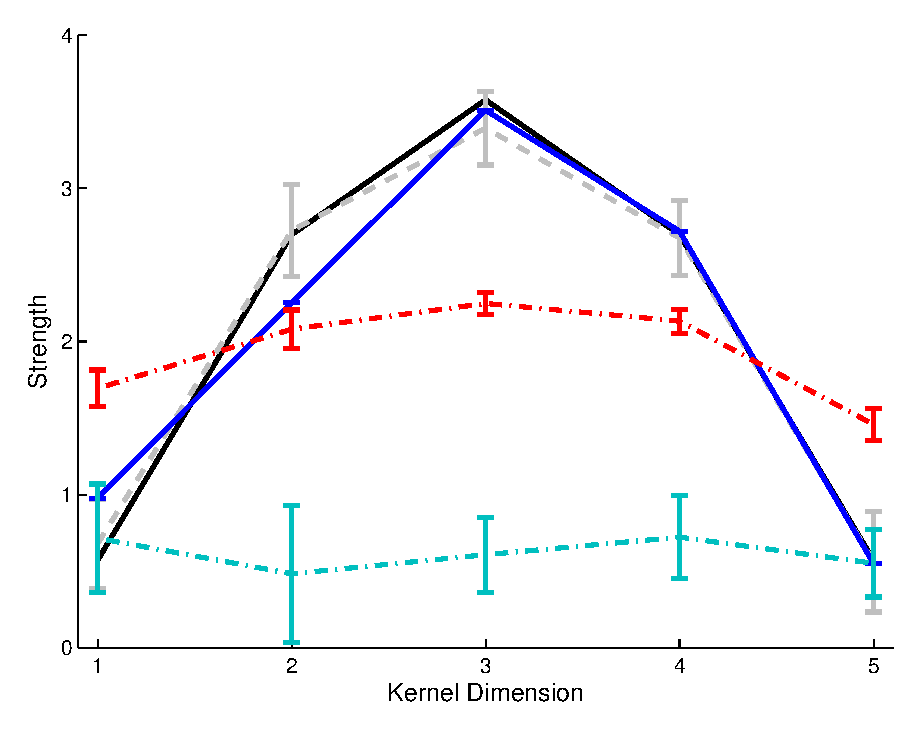
\includegraphics[width=.9\linewidth]{../figs/kernel}
\caption{The tuning curve of a neuron (black line), estimating from the true spike train (gray line), and the inferred spike train using the (i) FAND filter (blue line), (ii) Wiener filter (red line), and (iii) dF/F.  Clearly, the FAND filter performs nearly as well as the true spike train, whereas the Wiener filter and dF/F do not.  Note that half-wave rectification of the Wiener did not change the results at all.  Simulation details: mean (solid lines) and standard deviation (bars) of 5 simulations,$T=800$, $\Del=0.005$ sec, $\alpha=1$, $\beta=0$, $\tau=0.1$ sec, $x_{i,t} \sim \mU(0,0.2)$,  $\sig=0.25$.} \label{fig:kernel}
\end{figure}


%The correlation coefficient between $\bn^{FAND}$ and $\bn$ versus $\bn^{Wiener}$ and $\bn$ for this example is $0.92$ versus $0.57$.  Thresholding $\bn^{Wiener}$ after inference improves the correlation coefficient to $0.69$.  Running this simulation many times demonstrates that these results are typical: $\bn^{FAND}$ always outperforms $\bn^{Wiener}$, whether or not it $\bn^{Wiener}$ thresholded.  

